

\tikzset{every picture/.style={line width=0.75pt}} %set default line width to 0.75pt        

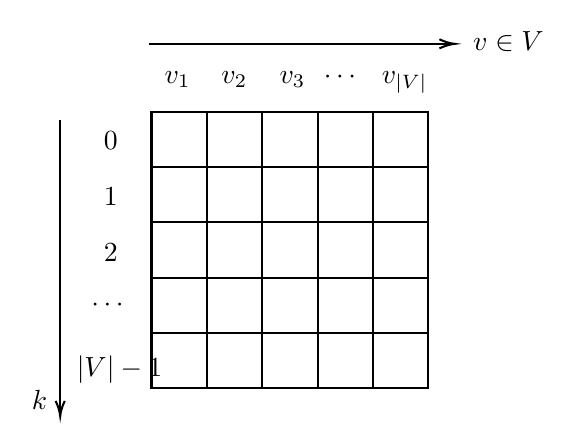
\begin{tikzpicture}[x=0.5pt,y=0.5pt,yscale=-1,xscale=1]
%uncomment if require: \path (0,320); %set diagram left start at 0, and has height of 320

%Shape: Grid [id:dp8546141469296037] 
\draw  [draw opacity=0] (107,81) -- (307,81) -- (307,281) -- (107,281) -- cycle ; \draw   (147,81) -- (147,281)(187,81) -- (187,281)(227,81) -- (227,281)(267,81) -- (267,281) ; \draw   (107,121) -- (307,121)(107,161) -- (307,161)(107,201) -- (307,201)(107,241) -- (307,241) ; \draw   (107,81) -- (307,81) -- (307,281) -- (107,281) -- cycle ;
%Straight Lines [id:da5603555662442616] 
\draw    (41,87) -- (41,299) ;
\draw [shift={(41,301)}, rotate = 270] [color={rgb, 255:red, 0; green, 0; blue, 0 }  ][line width=0.75]    (10.93,-3.29) .. controls (6.95,-1.4) and (3.31,-0.3) .. (0,0) .. controls (3.31,0.3) and (6.95,1.4) .. (10.93,3.29)   ;
%Straight Lines [id:da2247331279399798] 
\draw    (105,32) -- (324,32) ;
\draw [shift={(326,32)}, rotate = 180] [color={rgb, 255:red, 0; green, 0; blue, 0 }  ][line width=0.75]    (10.93,-3.29) .. controls (6.95,-1.4) and (3.31,-0.3) .. (0,0) .. controls (3.31,0.3) and (6.95,1.4) .. (10.93,3.29)   ;

% Text Node
\draw (70.24,93.06) node [anchor=north west][inner sep=0.75pt]   [align=left] {$\displaystyle 0$};
% Text Node
\draw (70.24,133.56) node [anchor=north west][inner sep=0.75pt]   [align=left] {$\displaystyle 1$};
% Text Node
\draw (70.24,174.06) node [anchor=north west][inner sep=0.75pt]   [align=left] {$\displaystyle 2$};
% Text Node
\draw (61.24,214.56) node [anchor=north west][inner sep=0.75pt]   [align=left] {$\displaystyle \cdots $};
% Text Node
\draw (50.74,255.06) node [anchor=north west][inner sep=0.75pt]   [align=left] {$\displaystyle |V|-1$};
% Text Node
\draw (18.24,280.06) node [anchor=north west][inner sep=0.75pt]   [align=left] {$\displaystyle k\ $};
% Text Node
\draw (114.24,49.56) node [anchor=north west][inner sep=0.75pt]   [align=left] {$\displaystyle v_{1}$};
% Text Node
\draw (155.24,49.56) node [anchor=north west][inner sep=0.75pt]   [align=left] {$\displaystyle v_{2}$};
% Text Node
\draw (197.24,49.56) node [anchor=north west][inner sep=0.75pt]   [align=left] {$\displaystyle v_{3}$};
% Text Node
\draw (229.24,49.56) node [anchor=north west][inner sep=0.75pt]   [align=left] {$\displaystyle \cdots $};
% Text Node
\draw (271.24,49.56) node [anchor=north west][inner sep=0.75pt]   [align=left] {$\displaystyle v_{|V|}$};
% Text Node
\draw (337.24,21.06) node [anchor=north west][inner sep=0.75pt]   [align=left] {$\displaystyle v\in V$};


\end{tikzpicture}

